\section{Theoretical Analysis}
\label{sec:theoretical}

\par In this section, the circuit shown in the previous figure is analysed theoretically.
\par Our approach begins with getting a smaller value for the voltage input in our circuit. As such, we used a transformer, with a ratio of turns in the primary and secondary circuits of $\frac{1}{10}$. As a consequence, because the input voltage amplitude is $V_s=230V$, this value will be lowered to $V_r=\frac{230}{10}V$, so that the circuit can then approximate to 12V. Although we already have a better value for the voltage input, it still is an AC input that needs to be converted to DC. In order to do this, we proceeded as described next.
\par Firstly, we used a full wave rectifier. As we said before, this circuit allows us to use the full length of the wave, converting the initial AC signal in an equal amplitude unidirectional current. Therefore, the wave format remains unchanged if the voltage is positive and gets reflected if the voltage is negative.
\par Secondly, we used a parallel of a capacitor and a resistor, in order to reduce the variaton of the voltage output, and make it closer to a DC one. This circuit is called an envelope detector, and it works based on the charge and discharge proccesses of the capacitor - when the diodes of the full-wave rectifier are on, the capacitor charges up, and when they turn off, the capacitor discharges through the resistor (in order to make things more clear, we're calling $v_O(env)$ to the voltage drop in $R_1$ terminals).
\par In order to compute the output of this process, we needed to know when the capacitor starts and stops discharging ($t_{off}$ and $t_{on}$, respectively). As one might guess, and based on what has been said, $t_{off}$ corresponds to the instant in which the diodes become off ($t_{off}=\frac{1}{\omega} \cdot atan(\frac{1}{\omega R_1C})$) and if $t<t_{off}$, $v_O(env)=v_R$. On the other hand, $t_{on}$ corresponds to the instant in which the diodes become on ($t{on}$ is obtained by solving the equation $Asin(\omega t{on})=Asin(\omega t_{off}) \cdot e^{-\frac{t_{on}-t_{off}}{R_1C}}$) and if $t<t_{on}$, $v_O(env)=Asin(\omega t_{off}) \cdot e^{-\frac{t-t_{off}}{R_1C}}$. The ripple voltage is given by max($v_O$(env)-min($v_O(env)$) and it's value is shown in the table bellow, as well as the average voltage output value. As we can see, the value of the ripple voltage is very low, which is very good. 

\vspace{5mm}
\begin{table}[H]
\centering
\begin{tabularx}{0.9\textwidth} {
  | >{\raggedright\arraybackslash}X
  | >{\raggedleft\arraybackslash}X | }
 \hline
\input{../mat/envelope_tab.tex}
\end{tabularx}
\caption{\label{tab:Table 1} Ripple and average value for the envelope detector (all values are in Volt)}
\end{table}
\vspace{5mm}

\par Thirdly, we used a series of 22 diodes, in series with a resistor (voltage regulator circuit) in order to "get rid" of the AC component and make the DC component 12V. This makes the current an almost perfect 12V DC, because the diodes have a constant voltage output, no matter what the current or voltage inputs are. If we compute the minimum value of $v_O(env)$, we can conclude if it sufices to turn the diodes on (this happens when $min(v_O(env)) \geq nv_{ON}$, being $v_{ON}$ the minimum voltage required to activate one diode).
\par At this point, we have the DC component of the voltage, so we need to calculate and minimize the AC component. This is achieved by making incremental analysis. In incremental analysis, we can replace each diode by a resistor with resistance $r_d$, and we get $v_o = \frac{n \cdot r_d}{n \cdot r_d+R_2} \cdot (v_O(env)-V_O(env))$. As we can see, if $R_2 \gg n \cdot r_d$, $v_o \approx 0$.
\par Putting all this things together, we get a final output voltage $v_O=V_O+v_o$, and the average of the signal must be approximatly 12V. The values of the ripple and average output voltage for the voltage regulator can be seen in the following table. As we can see, the value of the ripple voltage is very low, which is very good. Although the average voltage output is indicated as being 12V exactly, it isn't exactly 12V, because of the approximation made by octave's output - the deviation is so small, that this value is rounded to exactly 12V.

\vspace{5mm}
\begin{table}[H]
\centering
\begin{tabularx}{0.9\textwidth} {
  | >{\raggedright\arraybackslash}X
  | >{\raggedleft\arraybackslash}X | }
 \hline
\input{../mat/regulator_tab.tex}
\end{tabularx}
\caption{\label{tab:Table 2} Ripple and average value for the voltage regulator (all values are in Volt)}
\end{table}
\vspace{5mm}

\par It is important to mention that for simplification, the four diodes used for the full wave rectifier, were assumed to be ideal diodes since the change in current and voltage in those diodes, doesn't affect in a big way the output ripple and voltage. 

\par In the following picture, the output voltage of the full-wave rectifier, output voltage of the envelope detector and output voltage of the voltage regulator are plotted. Here we have a more visual perception of the values shown in the previous tables. The ripple of the final output (blue line) is even lower than the ripple of the envelope detector's output (green line) but as this value was already very low, it is not noticeable and the output looks like a straight line (although it isn't). In the last two plots we can see by the sacale used that the ripple in both the envelope detector and the voltage regulator are in fact very small.

\begin{figure}[H] \centering
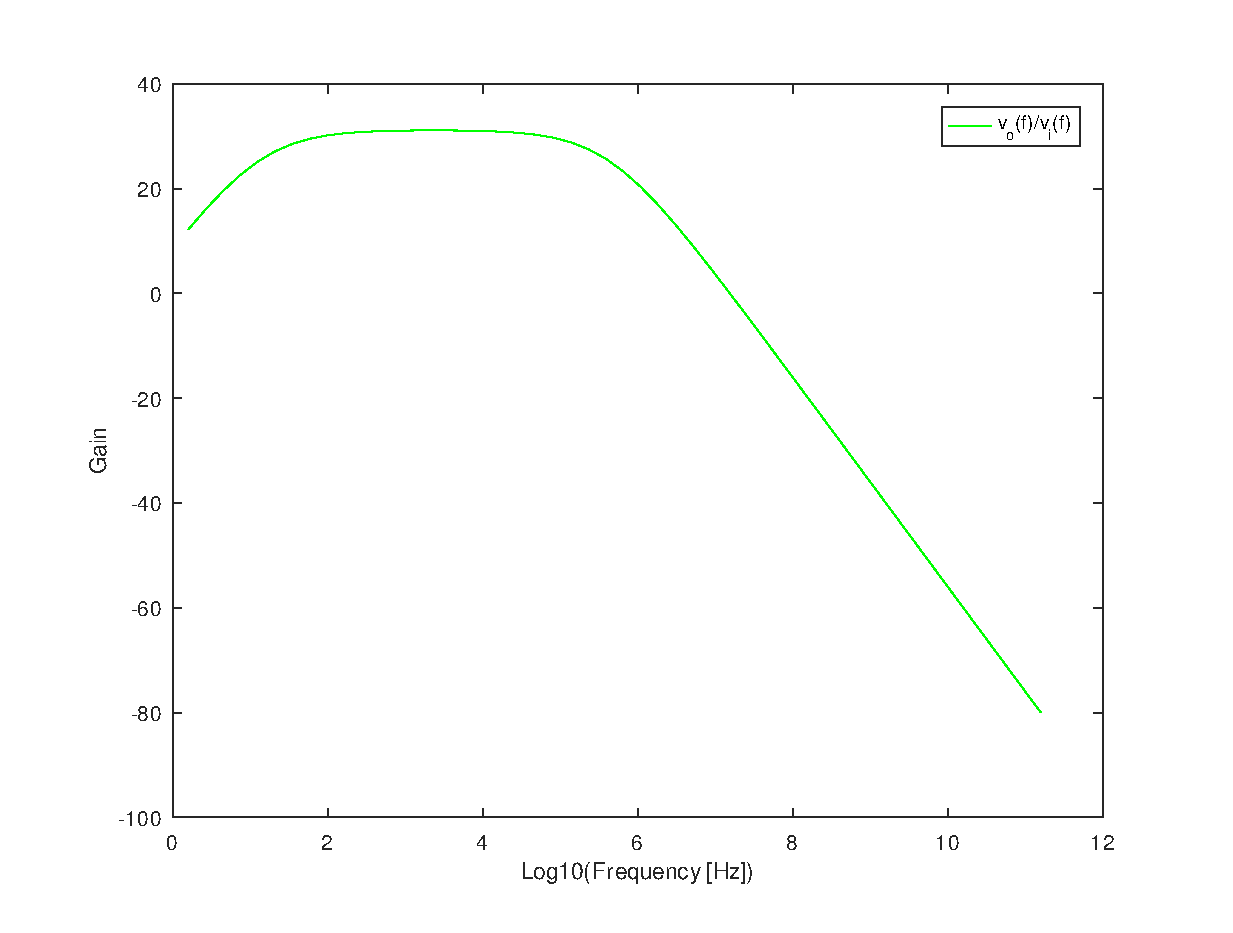
\includegraphics[width=1\linewidth]{teoria.eps}
\caption{Input voltage of the secondary circuit, output voltage of the envelope detector and output voltage of the voltage regulator}
\end{figure}

\begin{figure}[H] \centering
\includegraphics[width=1\linewidth]{ripple_env.eps}
\caption{Ripple of the voltage output in the envelope detector}
\end{figure}

\begin{figure}[H] \centering
\includegraphics[width=1\linewidth]{ripple_reg.eps}
\caption{Ripple of the voltage output in the voltage regulator}
\end{figure}


\par Lastly, the parameters used can be seen in the following table. The method through which we obtained this values will be explained in the next section.

\vspace{5mm}
\begin{table}[H]
\centering
\begin{tabularx}{0.9\textwidth} {
  | >{\raggedright\arraybackslash}X
  | >{\raggedleft\arraybackslash}X | }
 \hline
R1 & 1.006765e+03 Ohm \\ \hline
R2 & 2.033032e+03 Ohm \\ \hline
R3 & 3.033913e+03 Ohm \\ \hline
R4 & 4.003128e+03 Ohm \\ \hline
R5 & 3.131011e+03 Ohm \\ \hline
R6 & 2.093899e+03 Ohm \\ \hline
R7 & 1.017744e+03 Ohm \\ \hline
Vs & 5.223200e+00 V \\ \hline
C & 1.035361e-06 F \\ \hline
Kb & 7.272764e-03 S \\ \hline
Kd & 8.170065e+03 Ohm \\ \hline

\end{tabularx}
\caption{\label{tab:Table 3} Parameters used in the circuit}
\end{table}
\vspace{5mm}
	


